\lstset{caption=Ejemplo Modelo VAR,framexleftmargin=5mm, frame=shadowbox, rulesepcolor=\color{green}}
\begin{lstlisting}[title={‘Código R: ejemplo Modelo VAR},basicstyle=\ttfamily]{}
 rm(list=ls())
install.packages(vars)
library(vars)
data("Canada")
summary(Canada)
plot(Canada, nc = 2, xlab = "")
adf2 <- summary(ur.df(Canada[, "prod"], type = "drift", lags = 1))
\end{lstlisting}
%\end{frame}


\begin{figure}[H]
	\centering
	\textbf{}\par\medskip
	\fcolorbox{green}{blue}{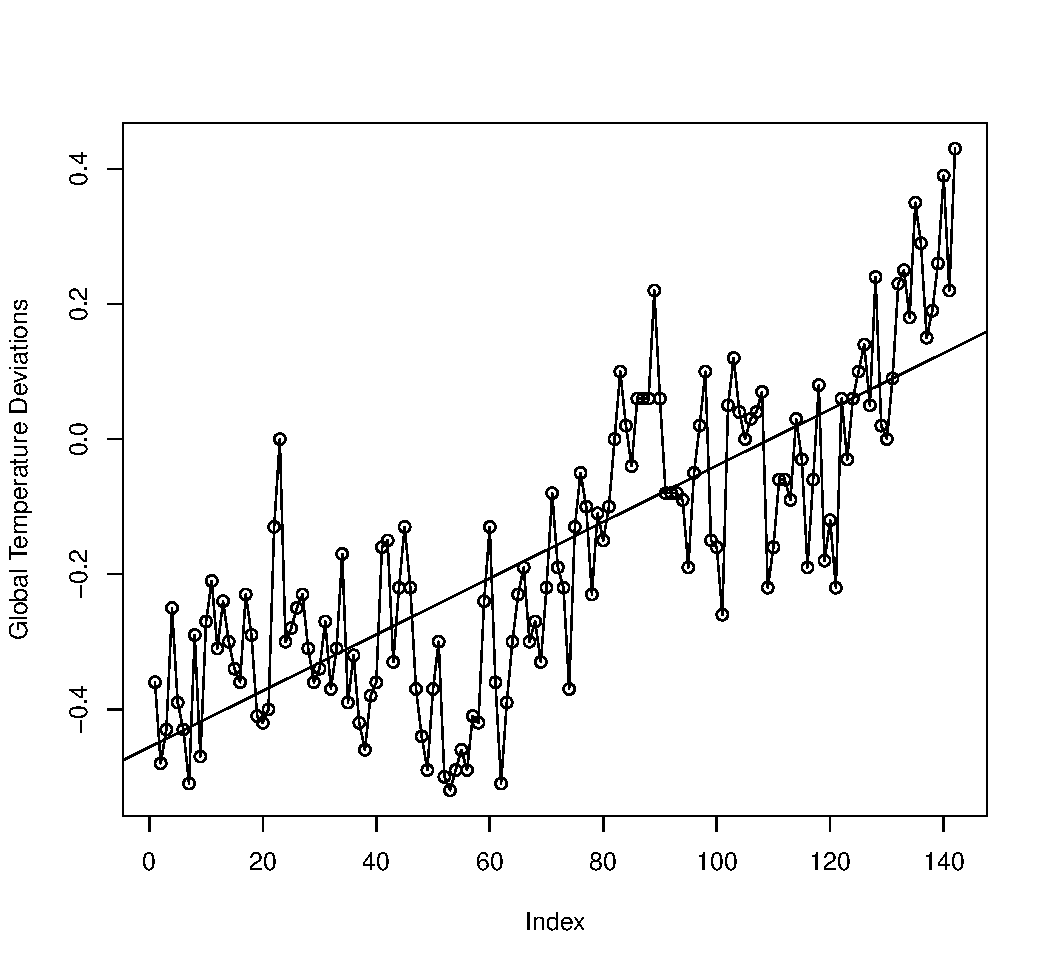
\includegraphics[width=\linewidth,scale=0.5]{gtemp_graph.pdf}}
	\caption{}\label{figxx}
\end{figure}

\begin{mdframed}[style=MyFrame]
\begin{definition}\label{def}
	\textbf{Definici\'on: operador de retroceso (backshift operator):}
		\begin{equation}
		B x_t = x_{t-1} 
		\end{equation}
		\begin{equation}
		B^2 x_t =  B(B x_t) = B x_{t-1} = x_{t-2}
		\end{equation}
		As\'{\i}:
		\begin{equation}
		B^k x_t = x_{t-k} 
		\end{equation} 
\end{definition}
\end{mdframed}
